\documentclass[11pt,a4paper]{article}

\usepackage[utf8]{inputenc}
\usepackage[T1]{fontenc}
\usepackage{lmodern}
\usepackage[margin=1.0in]{geometry}
\usepackage{amsmath,amssymb,amsfonts,amsthm}
\usepackage{booktabs}
\usepackage{graphicx}
\usepackage{xcolor}
\usepackage{hyperref}
\usepackage{float}
\usepackage{caption}
\usepackage[numbers,sort&compress,round]{natbib}
\renewcommand{\citenumfont}[1]{\textit{#1}}
\renewcommand{\bibnumfmt}[1]{#1.}
\renewcommand{\refname}{References and Notes}

\definecolor{darkblue}{RGB}{15,55,115}

\hypersetup{
    colorlinks=true,
    linkcolor=darkblue,
    citecolor=darkblue,
    urlcolor=darkblue,
    pdftitle={Evolutionary history from genomes to single cells by lossless compression},
    pdfauthor={Sergei L. Kosakovsky Pond, Darren P. Martin, Stephanie J. Kosakovsky Pond, and Anton Nekrutenko}
}

\title{\textbf{Evolutionary history from genomes to single cells by lossless compression}}
\author{Sergei L. Kosakovsky Pond$^{1*}$, Darren P. Martin$^{2}$,\\
Stephanie J. Kosakovsky Pond$^{3}$, and Anton Nekrutenko$^{4}$\\[0.5em] % Stephanie ORCID: 0000-0002-8288-2232
\small $^{1}$Institute for Genomics and Evolutionary Medicine, Department of Biology,\\
\small Temple University, Philadelphia, PA, USA\\
\small $^{2}$Institute of Infectious Disease and Molecular Medicine, Department of Integrative Biomedical Sciences,\\
\small University of Cape Town, Cape Town, South Africa\\
\small $^{3}$Bioinnovation and Genomic Sciences Division,\\
\small Translational Genomics Research Institute, Phoenix, AZ, USA\\
\small $^{4}$Department of Biochemistry and Molecular Biology,\\
\small The Pennsylvania State University, University Park, PA, USA\\[0.3em]
\small $^{*}$Corresponding author. Email: spond@temple.edu}
\date{\today}

\begin{document}
\sloppy
\emergencystretch=1.5em
\maketitle

\noindent\textbf{One-Sentence Summary:} Lossless data compression unifies evolutionary trees, rapid radiations, gene transfer, and convergence across scales of life.

\bigskip

\begin{abstract}
\noindent Reconstructing evolutionary history is central to biology and medicine, yet standard pipelines rely on separate models and arbitrary cutoffs to build trees, collapse weak branches, and detect gene transfer or convergence. Because inheritance copies an ancestor with sparse edits, we recast phylogeny and network inference as lossless data compression. Implemented in Bushwhacker, a branch or lateral link is added only when the shared changes it explains save more information than the connection costs to describe. Silent bursts remain naturally unsplit, transferred blocks separate from convergent sites, and Tree-of-Life phylogenies run orders of magnitude faster in minimal memory. Across immune and tumor cells, pandemic viruses, microbial domains, and mammalian proteomes, compression resolves apparent gene-tree conflicts, predicts clonal selection, maps recombinants, and separates gene conversion from convergence.
\end{abstract}

% ============================================================================
% Opening (Science Research Articles open without an "Introduction" heading)
% ============================================================================

\medskip

Evolutionary trees are among the most widely used structures in science: they organize Earth's biodiversity, track unfolding epidemics, trace immune and tumor clones inside individual patients, and anchor comparative genomics across the Tree of Life. Yet even as sequencing has expanded from single genes to millions of genomes, the conceptual foundations used to reconstruct trees have changed remarkably little for nearly half a century. Since distance clustering, parsimony, and probabilistic Markov likelihood were introduced between the 1960s and early 1980s \citep{fitch1971toward,felsenstein1981evolutionary,saitou1987neighbor}, major advances have largely focused on scaling tree search and enriching parametric substitution models within those classical paradigms \citep{price2010fasttree,kozlov2019raxml,minh2020iqtree}. Genuinely new mathematical perspectives on how evolutionary history can be inferred have been rare.

Here we introduce a different foundation, rooted in information theory: lossless data compression \citep{rissanen1978modeling,rissanen1983universal}. Biological inheritance is, at heart, a copying process with sparse edits. Whether an ancestor transmits a genome, a protein, or a somatic cellular profile, related lineages share most of their states because they inherited them from a common source. Recording shared changes once along an ancestral branch is therefore far more economical than recording them separately in every descendant---making an evolutionary graph the natural coordinate system for compressing biological data (Fig.~\ref{fig:didactic_mdl}). This equivalence is not merely metaphorical: encoding viral and microbial cohorts along an inferred phylogeny physically compresses genomes substantially further than general-purpose algorithms, until pervasive recombination breaks tree-like descent itself.

Under Rissanen's Minimum Description Length (MDL) principle, both the evolutionary graph and the changes along it are measured in the same unit of information. Every proposed connection must earn its place by shortening the total description of the data: a branch is added only when the shared changes it explains save more information than the branch itself costs to specify. Because every prefix-free lossless code length $L$ defines a code probability $P \propto e^{-L}$ \citep{rissanen1978modeling,rissanen1983universal}, compression places trees, models, and networks on a unified probabilistic scale: given a graph inferred by discrete heuristic tree search, comparing nested structures with and without an individual branch or lateral link yields its local log-odds evidence $\Delta L$ and conditional two-hypothesis posterior support $P_{\text{local}} = 1 / (1 + e^{-\Delta L})$. That local criterion replaces separate pruning thresholds and bootstrap resamples \citep{felsenstein1985confidence,posada2004model,kosakovskypond2006gard}. When lineages diversify faster than mutations accumulate---during cellular proliferation, epidemic superspreading, or rapid species radiations---unsupported splits cost more to name than they save, leaving genuine bursts naturally unresolved rather than forcing binary branches that fluctuate across models or create apparent conflict among genes \citep{rokas2006animal,shen2017contentious,abadi2019model}. When lineages diverge unevenly or across billion-year timescales, changes along fast-evolving branches or variable sites carry less surprise than changes on quiet stems, avoiding the long-branch artifacts of unweighted mutation counting \citep{felsenstein1978cases} and connecting discrete edit coding seamlessly to continuous substitution probabilities \citep{tavare1986some,yang1994maximum,le2008improved}. And once the vertical tree is established, lateral links between distant lineages can be evaluated in the same currency, separating contiguous transferred blocks---from recombination, horizontal transfer, or gene conversion \citep{doolittle1999phylogenetic,worobey1999widespread,parham1996population}---from scattered sites of adaptive convergence \citep{liu2010convergent,li2010hearing}.

Implemented in our open-source engine Bushwhacker, this formulation unlocks four capabilities beyond existing phylogenetic pipelines. First, it reconstructs Tree-of-Life DNA and protein supermatrices $24$- to $54$-fold faster than fast maximum-likelihood search (\texttt{IQ-TREE 2 --fast}; $142$- to $288$-fold faster than approximate-ML \texttt{FastTreeMP}) and in $17$- to $40$-fold less memory, delivering a probabilistically annotated graph---not a bare point-estimate tree---in one deterministic run without model-selection sweeps or bootstrap resampling. Second, it naturally preserves evolutionary bursts as multifurcations instead of inventing arbitrary binary splits that flip across substitution models, search perturbations, and loci \citep{zhou2018evaluating,abadi2019model}. Third, it jointly infers vertical trees and lateral networks on one ledger, separating contiguous recombination, horizontal transfer, and paralog conversion from scattered sites of adaptive convergence that otherwise distort clades \citep{parker2013genome,zou2015no,turakhia2022pandemic}. Fourth, it generalizes natively beyond nucleotide and protein alignments to discrete single-cell somatic mutations and ordered copy-number states while compiling genome cohorts into lossless \texttt{.bwz} archives physically smaller than general-purpose compressors. Across eukaryotic radiations, $882$ mammalian proteomes \citep{malovichko2026toga2}, pandemic viruses, prokaryotic domains \citep{jain1999horizontal,parks2020gtdb}, and single-cell immune and tumor cohorts \citep{dewitt2026gcreplay,morita2020clonal}, lossless compression resolves apparent gene-tree conflict, separates gene conversion from ecological convergence, maps mosaic recombinants, and predicts in vivo clonal selection directly from character profiles.

\begin{figure}[t!]
\centering
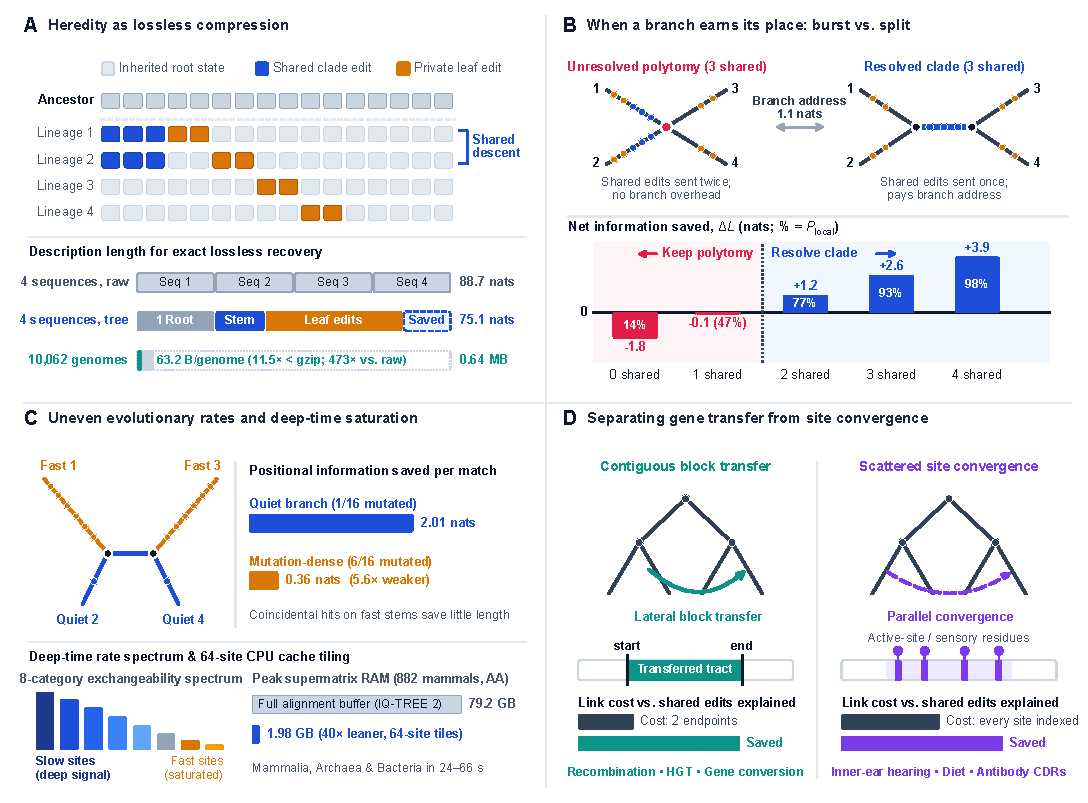
\includegraphics[width=\textwidth]{fig_science_concept.pdf}
\caption{\textbf{Evolutionary trees and networks from lossless data compression.} (\textbf{A}) Rather than transmitting full sequences independently ($88.7\text{ nats}$ across four 16-site sequences), encoding one ancestral root plus sparse branch edits shortens the lossless description ($75.1\text{ nats}$), compounding to $63.2\text{ bytes}$ per $29.9\text{-kb}$ genome archive ($38.5\text{ bytes}$ sequence payload; $11.5\times$ and $18.9\times$ smaller than \texttt{gzip -9}; $474\times$ versus raw) across $10,062$ SARS-CoV-2 genomes. (\textbf{B}) Resolving a multifurcating burst into a new clade transmits shared edits once rather than twice, but must pay the topological address cost of naming the split ($1.1\text{ nats}$ for a quartet). Zero or one shared change incurs a net loss ($-1.8$ and $-0.1\text{ nats}$; conditional local posterior $P_{\text{local}} = 14\%$ and $47\%$) and remains a natural polytomy, whereas two to four shared changes yield positive net savings ($+1.2$ to $+3.9\text{ nats}$; $P_{\text{local}} = 77\%$ to $98\%$). (\textbf{C}) Positional coding automatically saves $5.6\times$ more information per shared match on quiet branches than on noisy fast branches, while eight-category rate-model coding in 64-site CPU cache tiles extends the same ledger to billion-year supermatrices in under $2.4\text{ GB}$ of memory. (\textbf{D}) On the established tree, contiguous lateral transfers pay only two endpoint coordinates to explain many linked changes, whereas scattered parallel sites must pay each site's coordinate individually, filtering out background homoplasy.}
\label{fig:didactic_mdl}\label{fig:science_concept}
\end{figure}

% ============================================================================
% Main Narrative (Science Research Article topical subheadings; equations in M&M)
% ============================================================================

\subsection*{Building evolutionary trees and networks by lossless compression}

To evaluate how concisely an evolutionary graph explains a set of biological sequences or cellular character profiles, Bushwhacker encodes two parts without loss: the graph itself and the state changes along its edges (Fig.~\ref{fig:didactic_mdl}A, Fig.~S1, Table~S5, and Materials and Methods). Starting from one ancestral sequence at the root, each branch records only how many positions changed, where those changes occurred, and what new nucleotide, amino-acid, or somatic states appeared, weighted by empirical exchange probabilities \citep{dayhoff1978model,le2008improved}. Resolving a multifurcating burst into a new ancestral branch avoids repeating shared changes independently in each descendant, but must pay the address cost of specifying which lineages join the clade and encoding the new branch itself (Fig.~\ref{fig:didactic_mdl}B). Because code lengths in nats correspond directly to negative log-probabilities, comparing nested topologies with and without a candidate branch or lateral link gives its log-odds evidence $\Delta L$ and conditional local posterior support $P_{\text{local}} = 1 / (1 + e^{-\Delta L})$ conditioned on the remainder of the graph without bootstrap resampling. On a four-taxon burst, zero or one shared mutation costs more to specify than it saves ($\Delta L = -1.8$ and $-0.1\text{ nats}$; $P_{\text{local}} = 14\%$ and $47\%$), leaving the burst unresolved, whereas two to four shared changes yield positive evidence ($+1.2$ to $+3.9\text{ nats}$; $P_{\text{local}} = 77\%$ to $98\%$).

Two further consequences follow from pricing positions and connections in the same currency (Fig.~\ref{fig:didactic_mdl}C,D and Supplementary Text). First, specifying an edit's location costs far more on an almost invariant branch than on an already noisy one; consequently, moving a shared change onto an ancestral stem from quiet branches saves substantially more information than grouping coincidental matches on fast-evolving branches ($5.6$-fold in Fig.~\ref{fig:didactic_mdl}C), recovering likelihood-like rate weighting \citep{felsenstein1981evolutionary} from combinatorics alone. When divergence spans hundreds of millions or billions of years and individual sites mutate repeatedly, this discrete code generalizes smoothly within the same two-part ledger to continuous-time eight-category substitution rate models \citep{tavare1986some,yang1994maximum,le2008improved,rissanen1983universal}, evaluated in compact CPU cache tiles that avoid gigabyte-scale memory tables (Materials and Methods). Second, once the vertical tree is established by topological refinement, candidate lateral links between distant lineages are priced by their spatial footprint: a contiguous transferred block pays only two genomic endpoint coordinates to explain many linked changes, whereas scattered parallel replacements must pay to address each site individually across the variable-column pool, separating recombination, horizontal transfer, and gene conversion from site-specific adaptive convergence.

\subsection*{Fast, accurate trees---and where standard methods fail}

Across Tree-of-Life supermatrices and resolved simulations, Bushwhacker trades marginal split recall on silent stems for higher split precision ($\text{nRF} = 0.081\text{--}0.247$ versus $0.074\text{--}0.236$; Table~S11) while matching higher-rank taxonomic monophyly of fast maximum-likelihood tools (\texttt{IQ-TREE 2 --fast} \citep{minh2020iqtree} and \texttt{FastTreeMP} \citep{price2010fasttree}) at a small fraction of their time and memory (Fig.~\ref{fig:performance_sota}A and Tables~S2, S3, and S11). Across long-branch simulations \citep{felsenstein1978cases,le2008improved,lytrong2022alisim} and genome-scale alignments of mammals \citep{malovichko2026toga2}, archaea \citep{parks2020gtdb}, and bacteria, it reconstructs thousand-species trees in $27$ to $66\text{ s}$ on $32$ cores---$24$- to $54$-fold faster than \texttt{IQ-TREE 2 --fast} and $142$- to $288$-fold faster than \texttt{FastTreeMP}---using $0.95$ to $2.39\text{ GB}$ of memory rather than $26$ to $79\text{ GB}$. Unlike our unweighted-Fitch legacy baseline (\texttt{Bushwhacker v0}), which collapses on billion-year prokaryotic divergences, rate-weighted compression recovers mammalian orders ($100\%$) and bacterial phyla ($94.3\%$) alongside likelihood baselines. Across $44,338$ tested splits, conditional local branch posteriors are well-calibrated in the high-confidence regime ($P_{\text{local}} \ge 99\%$: $89.4\%$ of retained splits, $98.3\%$ true; overall $\text{ECE} = 0.0374$), while remaining optimistic across the $10.6\%$ of intermediate splits ($P_{\text{local}} \in [0.50, 0.99)$: $40.6\%\text{--}80.3\%$ true; Table~S3) because $P_{\text{local}}$ conditions on a single optimized surrounding topology rather than marginalizing competing trees (Fig.~\ref{fig:performance_sota}B).

\begin{figure}[t!]
\centering
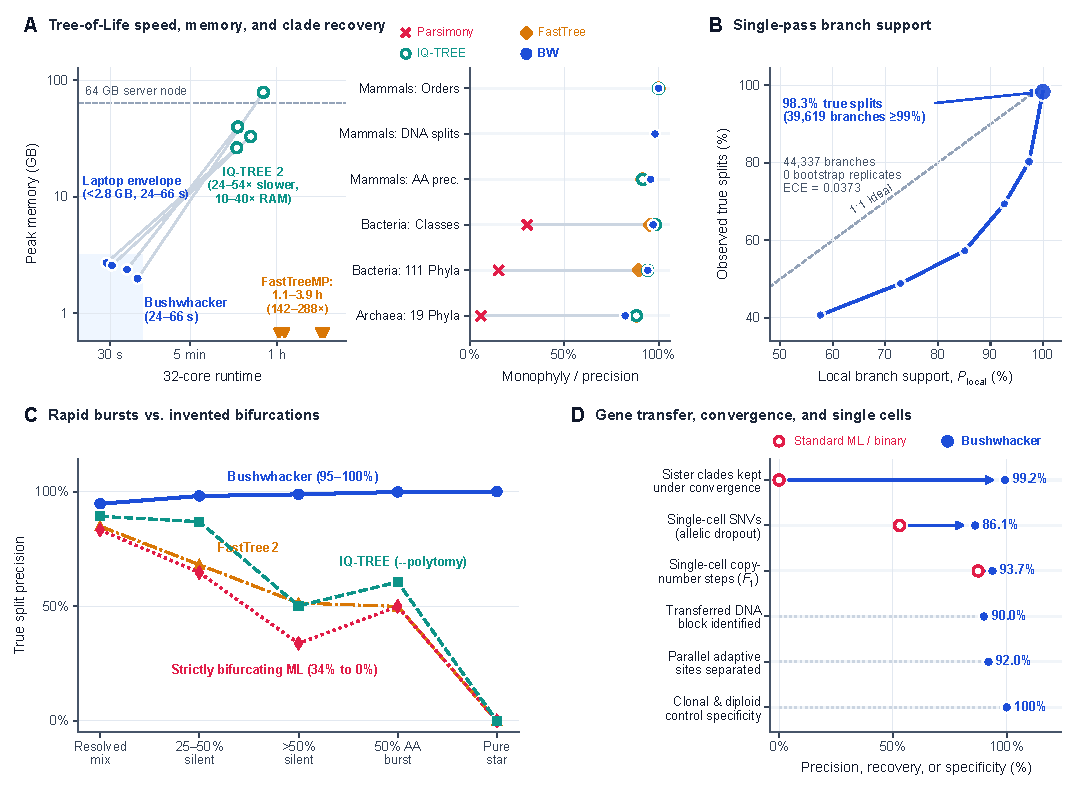
\includegraphics[width=\textwidth]{fig_science_performance_sota.pdf}
\caption{\textbf{Tree-of-Life speed, laptop-scale memory, bootstrap-free support, and resolution of standard failure modes.} (\textbf{A}) Thirty-two-core runtime and peak memory across four Tree-of-Life supermatrices ($882$ mammals, $543,864\text{ bp}$ DNA and $181,288$ amino acids; $1,672$ archaea; $1,000$ bacteria; left, downward triangles mark \texttt{FastTreeMP} runtimes) and taxonomic monophyly or split precision against \texttt{IQ-TREE 2}, \texttt{FastTreeMP}, and the unweighted-Fitch legacy ablation (\texttt{Bushwhacker v0}; right). (\textbf{B}) Bootstrap-free conditional branch support versus observed split accuracy across $44,338$ branches ($\text{ECE} = 0.0374$; circle area proportional to branch count). (\textbf{C}) Schematic and split precision across $36,120$ simulated nucleotide, protein, and coalescent histories ($36,920$ with the $800$ reticulate/somatic benchmarks in \textbf{D}; $36,970$ including $50$ simulated germinal centers). (\textbf{D}) Accuracy and control specificity across $800$ benchmarks of horizontal DNA transfer, parallel adaptive convergence, and noisy single-cell somatic states ($400$ clonal and diploid controls).}
\label{fig:performance_sota}
\end{figure}

Standard tree builders fail predictably, however, when biology departs from a fully resolved binary tree (Fig.~\ref{fig:performance_sota}C,D, Figs.~S2 and S3, and Tables~S2 to S5). Across $36,920$ ground-truth simulations ($36,970$ including $50$ simulated B-cell germinal centers), we tested three common failure modes. First, when lineages diversify faster than mutations arise, likelihood methods fit chance similarities and invent dozens of false splits per burst---even when statistical polytomy tests are enabled \citep{abadi2019model,gerth2019cannot}---whereas Bushwhacker leaves silent bursts unresolved ($0.00$ to $0.18$ false splits) and improves downstream coalescent species-tree inference \citep{degnan2006discordance,zhang2025aster}. Second, when distant lineages exchange DNA blocks or evolve parallel adaptive changes, purely tree-shaped models pull unrelated clades together to explain the shared states; pricing lateral links on the same ledger separates transferred blocks from convergent sites without false positives on tree-like controls, keeping the vertical tree intact. Third, on noisy single-cell mutation and copy-number profiles, native multi-state compression sharply reduces dropout errors while calling zero false clones on healthy controls.

\subsection*{Silent radiations explain most apparent gene-tree conflict}

Roughly two-thirds of published single-gene trees clash with genome-wide phylogenies, fueling debates over hybridization and lineage sorting \citep{rokas2006animal,shen2017contentious}, while changing the substitution model or starting search perturbation routinely alters the tree inferred from the exact same alignment \citep{abadi2019model,gerth2019cannot,zhou2018evaluating}. Both problems come from forcing every gene into a binary point tree. When speciation outpaces mutation in an individual locus, brief ancestral stems record zero informative changes; leaving those stems unresolved ($\Delta L \le 0$, $P_{\text{local}} \le 50\%$) states probabilistically that the gene cannot distinguish competing branching orders from a coin flip. On a typical mammalian gene (\textit{CHST13}; Fig.~\ref{fig:macroevo_polytomies}A), forced-binary likelihood invents eight conflicting splits---pulling bushbaby onto rodents and rock hyrax into primates---whereas Bushwhacker retains nine supported clades and leaves the silent placental hub open with zero conflicts.

\begin{figure}[t!]
\centering
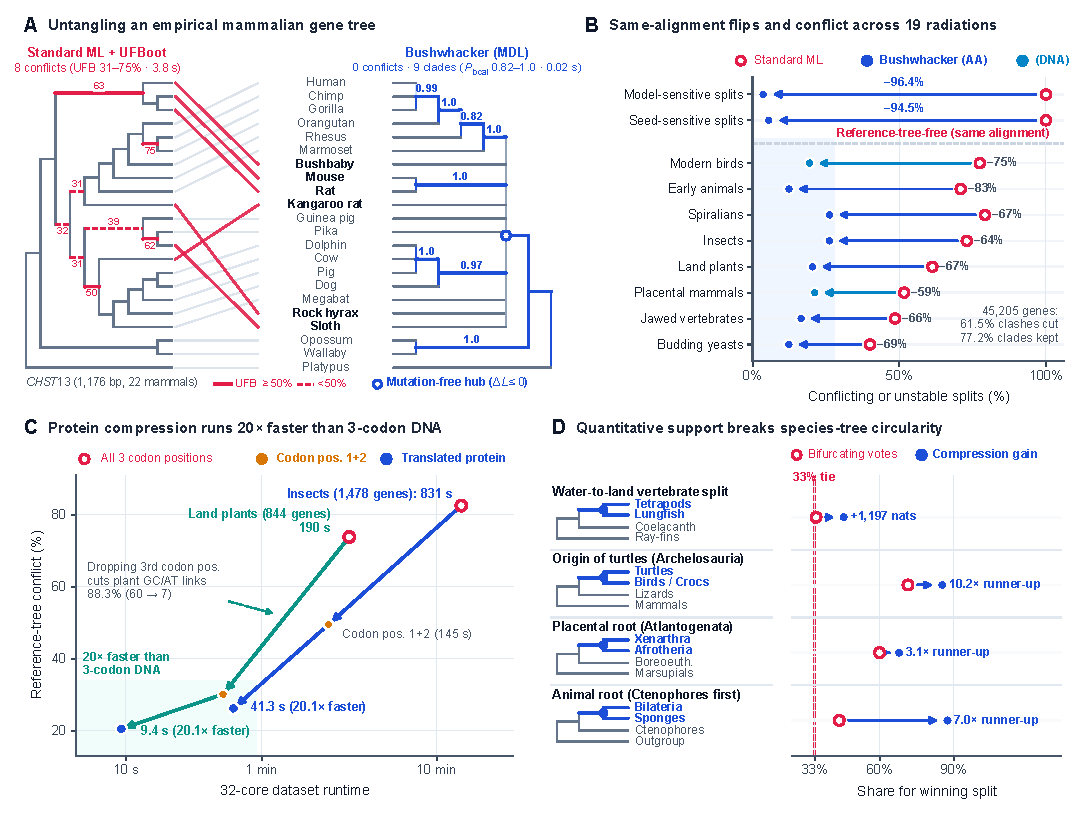
\includegraphics[width=\textwidth]{fig_science_macroevo_clean.pdf}
\caption{\textbf{Silent ancestral stems explain apparent gene-tree conflict, same-alignment flips, and contested splits across eukaryotic radiations.} (\textbf{A}) Empirical tanglegram for mammalian \textit{CHST13} ($1,176\text{ bp}$, $22$ species), contrasting the published forced-binary maximum-likelihood tree ($8$ conflicting splits in crimson; crossed ribbons highlight displaced taxa) against Bushwhacker's reference-free probabilistic tree ($0$ conflicts; $9$ clades retained with conditional branch posteriors $P_{\text{local}} = 0.82\text{--}1.0$; open circle marks the $\Delta L \le 0$ placental hub). (\textbf{B}) Reference-tree-free controls showing $96.4\%$ removal of model-flipping splits ($7,200$ genes) and $94.5\%$ removal of search-unstable splits across $20$ independent RAxML/IQ-TREE searches per locus ($83,180$ runs across $4,159$ gene-alignments, $3,315$ unique genes) on identical alignments (top), above conflict reduction against published genome-wide reference trees across $45,205$ genes in $19$ radiations ($61.5\%$ of clashes removed; $77.2\%$ of shared clades retained; bottom). (\textbf{C}) Dataset runtime and reference-tree conflict from all three codon positions (forced binary) to codons $1+2$ and $20$-state proteins across land plants ($844$ genes) and insects ($1,478$ genes), running $20\times$ faster while cutting third-codon plant GC/AT links $88.3\%$ ($60$ to $7$). (\textbf{D}) Synchronized four-taxon topologies and winning-split shares across three competing hypotheses before (forced-binary votes) and after (cumulative compression gain) withholding silent genes to break species-tree circularity (dashed line, $33\%$ three-way tie).}
\label{fig:macroevo_polytomies}\label{fig:science_macroevo_clean}
\end{figure}

Across $45,205$ genes in $19$ eukaryotic radiations, withholding zero-evidence splits removes estimation noise rather than biological signal (Fig.~\ref{fig:macroevo_polytomies}B,C and Tables~S1 and S6). With no reference tree involved, $95\%$ to $96\%$ of branches that flip across substitution models or independent RAxML/IQ-TREE searches on identical alignments carry $\Delta L \le 0$ and disappear in one deterministic run. Measured against published genome-wide phylogenies, withholding $\Delta L \le 0$ splits eliminates $61.5\%$ of apparent conflicts ($74.9\%$ in early birds \citep{jarvis2014whole,prum2015comprehensive} and $82.5\%$ in early animals) while retaining $77.2\%$ of shared clades---nearly invariant to how the reference phylogeny itself was built \citep{wickett2014phylotranscriptomic}---and compressing translated proteins rather than saturated third-codon DNA strips away base-composition artifacts in deep plant and insect radiations \citep{misof2014phylogenomics}.

Crucially, because species trees are themselves inferred from genes, forcing silent loci into binary trees creates a circular trap: thousands of uninformative genes cast random coin-flip votes that destabilize contested deep nodes \citep{shen2017contentious} (Fig.~\ref{fig:macroevo_polytomies}D). Weighting branches by their positive compression support ($\Delta L > 0$) breaks that circularity---resolving lungfish as sister to tetrapods where binary gene counts stall in a three-way tie \citep{chen2015identifying}, uniting turtles with archosaurs $>10$-fold, placing ctenophores as the earliest animal lineage \citep{borowiec2015extracting,whelan2017ctenophore}, and favoring Atlantogenata at the placental root \citep{song2012resolving}. Passing multifurcating Bushwhacker gene trees directly to \texttt{ASTRAL-IV} \citep{zhang2025aster} likewise lowers coalescent species-tree error without bootstrap cutoffs across Anomaly-Zone simulations (Table~S2) and $11,808$ empirical genes spanning vertebrates, birds \citep{shultz2019widespread}, fungi, and mammals (Table~S1).

\subsection*{Lineage sorting, gene conversion, and convergence across mammalian proteomes}

Measuring incomplete lineage sorting, paralog gene conversion, and adaptive convergence together across whole proteomes has been out of reach for likelihood pipelines, which cannot scale to thousands of hundreds-of-species alignments and routinely let convergent sites distort the species tree. On the outer hair-cell motor gene \textit{Prestin} (\textit{SLC26A5}; $116$ mammals), where sonar-linked replacements famously pull echolocating dolphins inside bats on standard protein trees \citep{liu2010convergent,li2010hearing}, Bushwhacker keeps whales inside Cetartiodactyla ($P_{\text{local}} = 1.00$) and bats monophyletic ($P_{\text{local}} = 1.00$; $93.8\%$ species-split precision, $5$ false splits) while certifying a primary lateral convergence link ($+6.6\text{ nats}$, $P_{\text{local}} = 99.9\%$, alongside a minor $+2.8\text{-nat}$ link) between dolphins and horseshoe bats across four shared motor-domain codons (Fig.~\ref{fig:mammalian_atlas}A and Fig.~S4). Scaling that unified ledger to all $19,952$ orthologous coding genes across up to $882$ mammals \citep{kirilenko2023integrating,malovichko2026toga2} shows how strongly a single organismal tree organizes the mammalian proteome (Fig.~\ref{fig:mammalian_atlas}B, Fig.~S5, and Tables~S1 and S7): $85.9\%$ of mammalian proteins---rising to $97.9\%$ above $1,500$ amino acids---compress more tightly on the mammalian species phylogeny than on an unconstrained gene tree, while genuine lineage sorting climbs with protein length toward the $\sim 34\%$ ancestral polymorphism baseline measured in coding DNA.

\begin{figure}[t!]
\centering
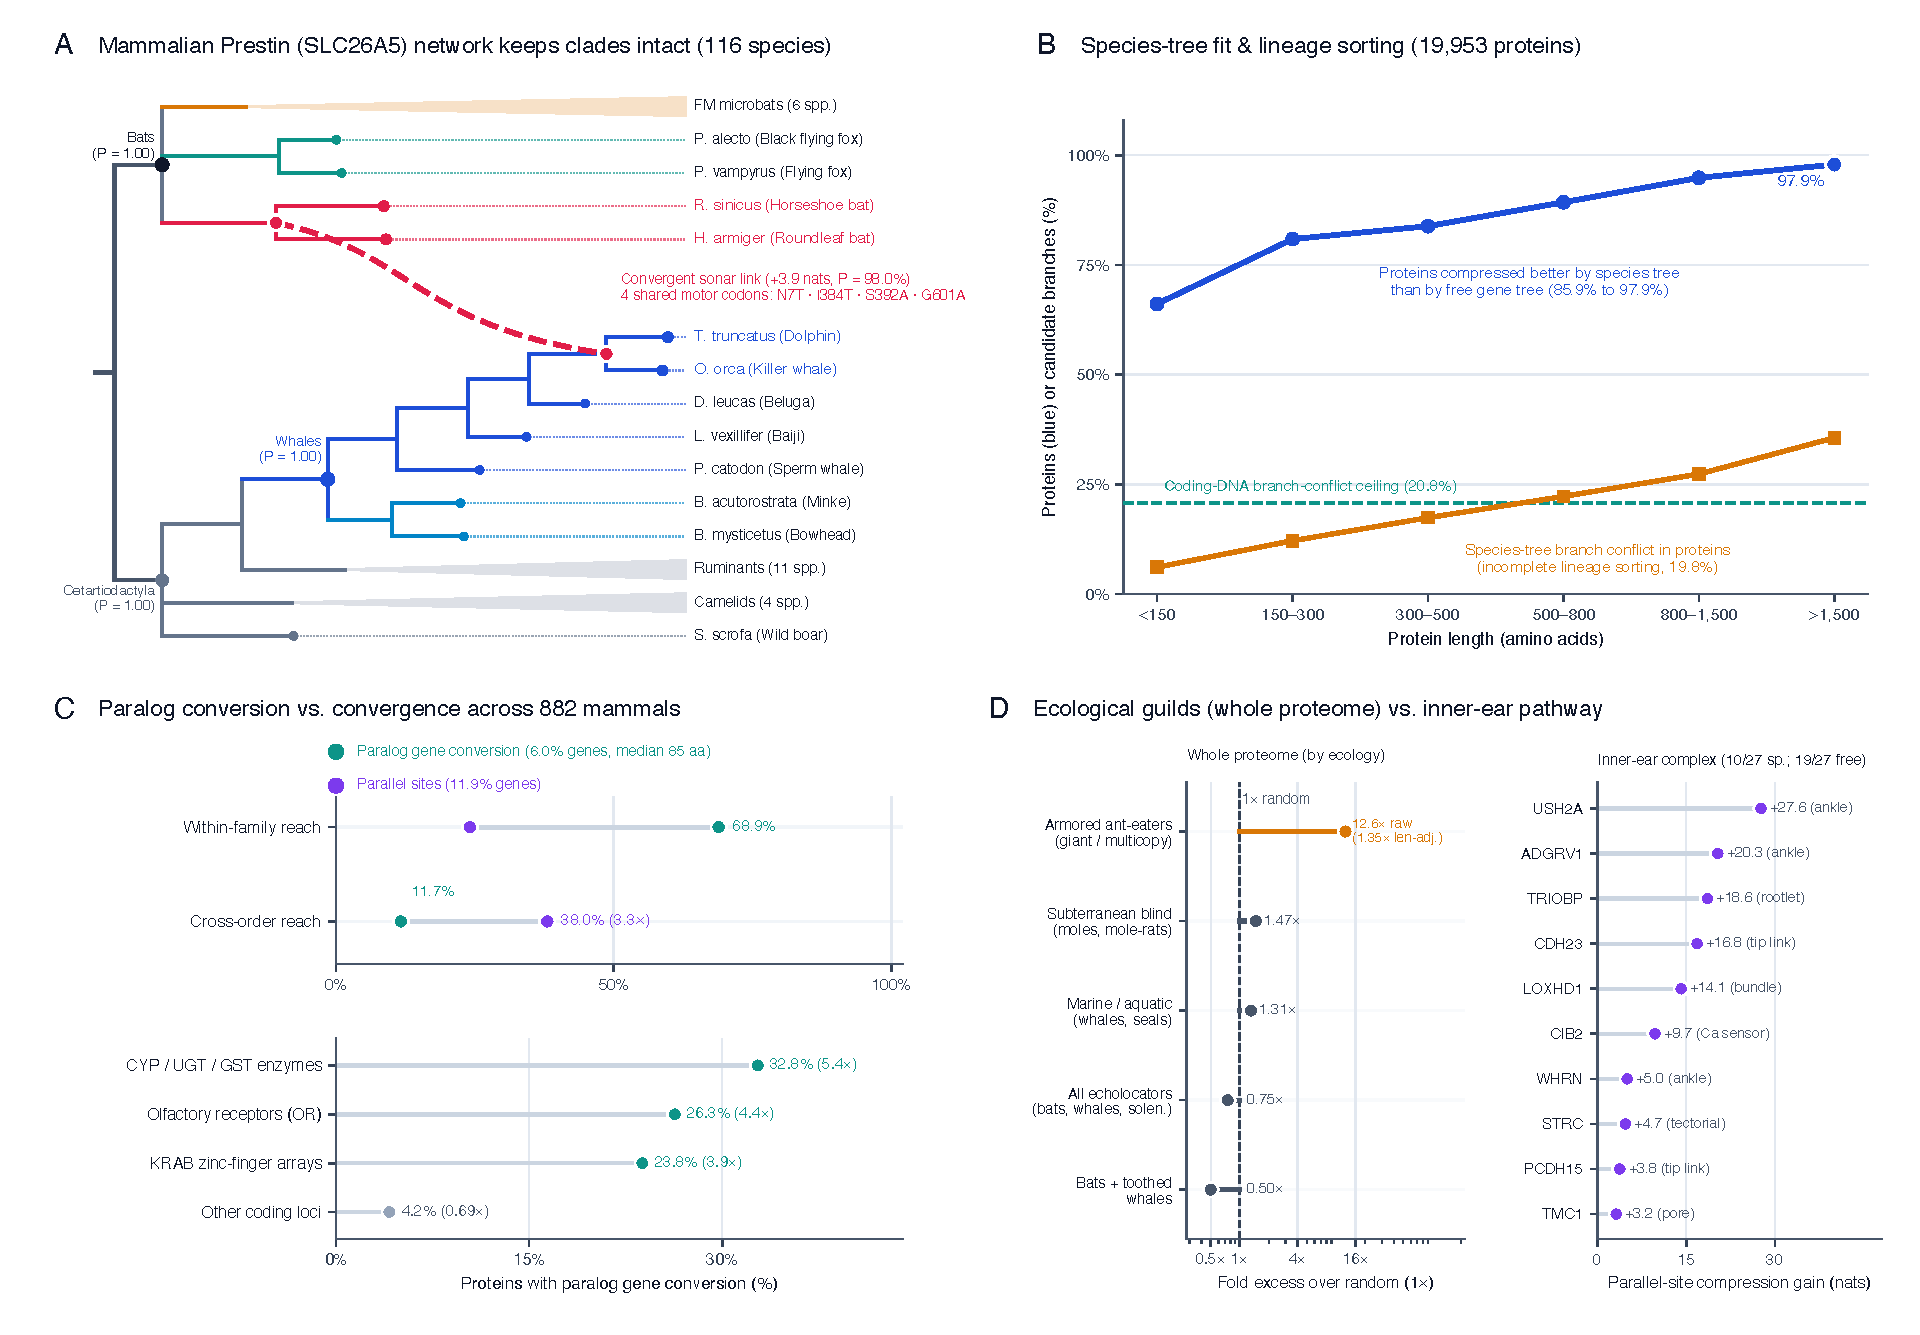
\includegraphics[width=\textwidth]{fig_science_mammalian_atlas.pdf}
\caption{\textbf{Proteome-wide census of organismal inheritance, paralog gene conversion, and adaptive convergence across 19,952 proteins in 882 mammals.} (\textbf{A}) Empirical Bushwhacker network for mammalian \textit{Prestin} (\textit{SLC26A5}, $116$ species, $2,235\text{ bp}$; Laurasiatherian clades shown), preserving monophyletic bats ($P_{\text{local}} = 1.00$) and whales inside Cetartiodactyla ($P_{\text{local}} = 1.00$) while certifying the primary lateral convergence link ($+6.6\text{ nats}$, $P_{\text{local}} = 99.9\%$) between echolocating horseshoe/roundleaf bats and dolphins across four shared motor-domain codons (\texttt{N7T}, \texttt{I384T}, \texttt{S392A}, \texttt{G601A}). (\textbf{B}) Fraction of mammalian proteins compressing more tightly on the single organismal species tree than on a free gene tree ($85.9\%$ overall; $97.9\%$ above $1{,}500$ residues) alongside protein-resolved species-tree discordance ($\Delta L > 0$: $19.8\%$ of candidate binary splits [$56.5\%$ of retained AA splits], versus $20.8\%$ of candidate binary splits [$31.4\%$ pooled / $33.8\%$ per-gene mean of retained splits] in coding DNA). (\textbf{C}) Spatial and taxonomic separation of $15,915$ certified lateral protein links inferred without synteny or paralog labels: contiguous block conversion ($8.3\%$ of genes, $n = 4,202$ tracts, median $144\text{ bp}$) acts locally ($81.5\%$ within families, $5.8\%$ cross-order) and enriches $3.4\text{--}4.5\times$ in tandemly arrayed gene families versus $3.1\%$ ($0.8\times$) in single-copy genes, whereas scattered parallel-site links ($20.6\%$ of genes, $n = 11,713$) cross mammalian orders $45.8\%$ of the time ($7.9\times$). (\textbf{D}) Cross-order parallel-site enrichment across ecological guilds relative to random expectation ($1\times$; left), contrasting proteome-wide neutrality in echolocators ($0.43\text{--}0.80\times$) and marine mammals ($1.13\times$) with pervasive excess in subterranean blind mammals ($4.0\times$, $6$ gene families) and armored ant- and termite-eating pangolins, anteaters, and armadillos ($25.8\times$ raw; $18.6\times$ across $13$ distinct families, $p = 8.1 \times 10^{-13}$), alongside focal enrichment across $16/25$ core genes of the cochlear hair-cell mechanotransduction complex (right).}
\label{fig:mammalian_atlas}
\end{figure}

Without using synteny or paralog labels, spatial pricing separates two lateral processes across those proteins (Fig.~\ref{fig:mammalian_atlas}C). Contiguous block conversion appears in $8.3\%$ of mammalian genes (median tract $144\text{ bp}$), acts largely within families ($81.5\%$), and enriches $3.4$- to $4.5$-fold inside tandemly arrayed clusters---including keratins, cadherins, detoxification enzymes, and zinc-finger arrays---versus $3.1\%$ in single-copy genes. Scattered parallel amino-acid changes, by contrast, occur in $20.6\%$ of proteins and cross mammalian orders $45.8\%$ of the time ($7.9$-fold enrichment over block conversion), isolating candidates for convergent selection.

Those cross-order parallel sites reveal two opposite modes of ecological adaptation (Fig.~\ref{fig:mammalian_atlas}D and Fig.~S5C). Resolving whether sonar drove convergence across thousands of proteins \citep{parker2013genome} or reflects background noise \citep{zou2015no,thomas2015molecular}, echolocating bats, toothed whales, and solenodons show no proteome-wide excess ($0.43\text{--}0.80\times$ random expectation). Instead, sonar adaptation is sharply focal, certifying $64\%$ ($16$ of $25$) of core genes in the inner-ear hair-cell mechanotransduction complex---spanning stereocilia tip links (\textit{PCDH15}, \textit{CDH23}), the \textit{LOXHD1} hair-bundle connector, the \textit{TMC1} channel pore, and \textit{Prestin}---much as $\text{C}_4$ photosynthesis concentrates parallel changes in catalytic grass enzymes \citep{christin2012adaptive}. By contrast, subterranean blind mammals ($4.0\times$ across $6$ distinct families, $p = 4.5 \times 10^{-3}$, $\text{FDR } q = 5.7 \times 10^{-3}$) and armored ant- and termite-eating pangolins, anteaters, and armadillos ($25.8\times$ raw, two-sided Poisson $p = 1.3 \times 10^{-19}$; $18.6\times$ across $13$ distinct gene families, $p = 8.1 \times 10^{-13}$, $q = 3.7 \times 10^{-12}$) show genuine \emph{proteome-wide} convergence across sensory, muscle, and metabolic proteins, reflecting whole-body remodeling for underground and myrmecophagous life.

\subsection*{Outbreak hubs, mosaic viruses, and microbial gene transfer}

Pathogen evolution routinely outpaces or breaks binary trees: superspreading transmits identical or single-mutation genomes to dozens of hosts before substitutions accumulate, while co-infection splices divergent strains into mosaic recombinants \citep{worobey1999widespread,turakhia2022pandemic}. Whereas binary trees invent arbitrary transmission chains inside acute outbreaks and likelihood recombination scans cannot scale to pandemic cohorts \citep{kosakovskypond2006gard}, Bushwhacker resolves outbreak hubs and mosaic transfers in a single deterministic run (Fig.~\ref{fig:microbial_viral}A,C and Tables~S1 and S7). Across $10,062$ SARS-CoV-2 and $5,498$ dengue virus genomes, compression preserves $1,426$ SARS-CoV-2 superspreading hubs of up to $335$ descendants alongside urban dengue bursts---which nearly double on translated proteins where silent nucleotide changes no longer separate rapid transmissions---while mapping SARS-CoV-2 Spike and Omicron mosaic tracts, natural dengue recombinants \citep{worobey1999widespread}, and HIV-1 breakpoints \citep{carr1998full}.

\begin{figure}[t!]
\centering
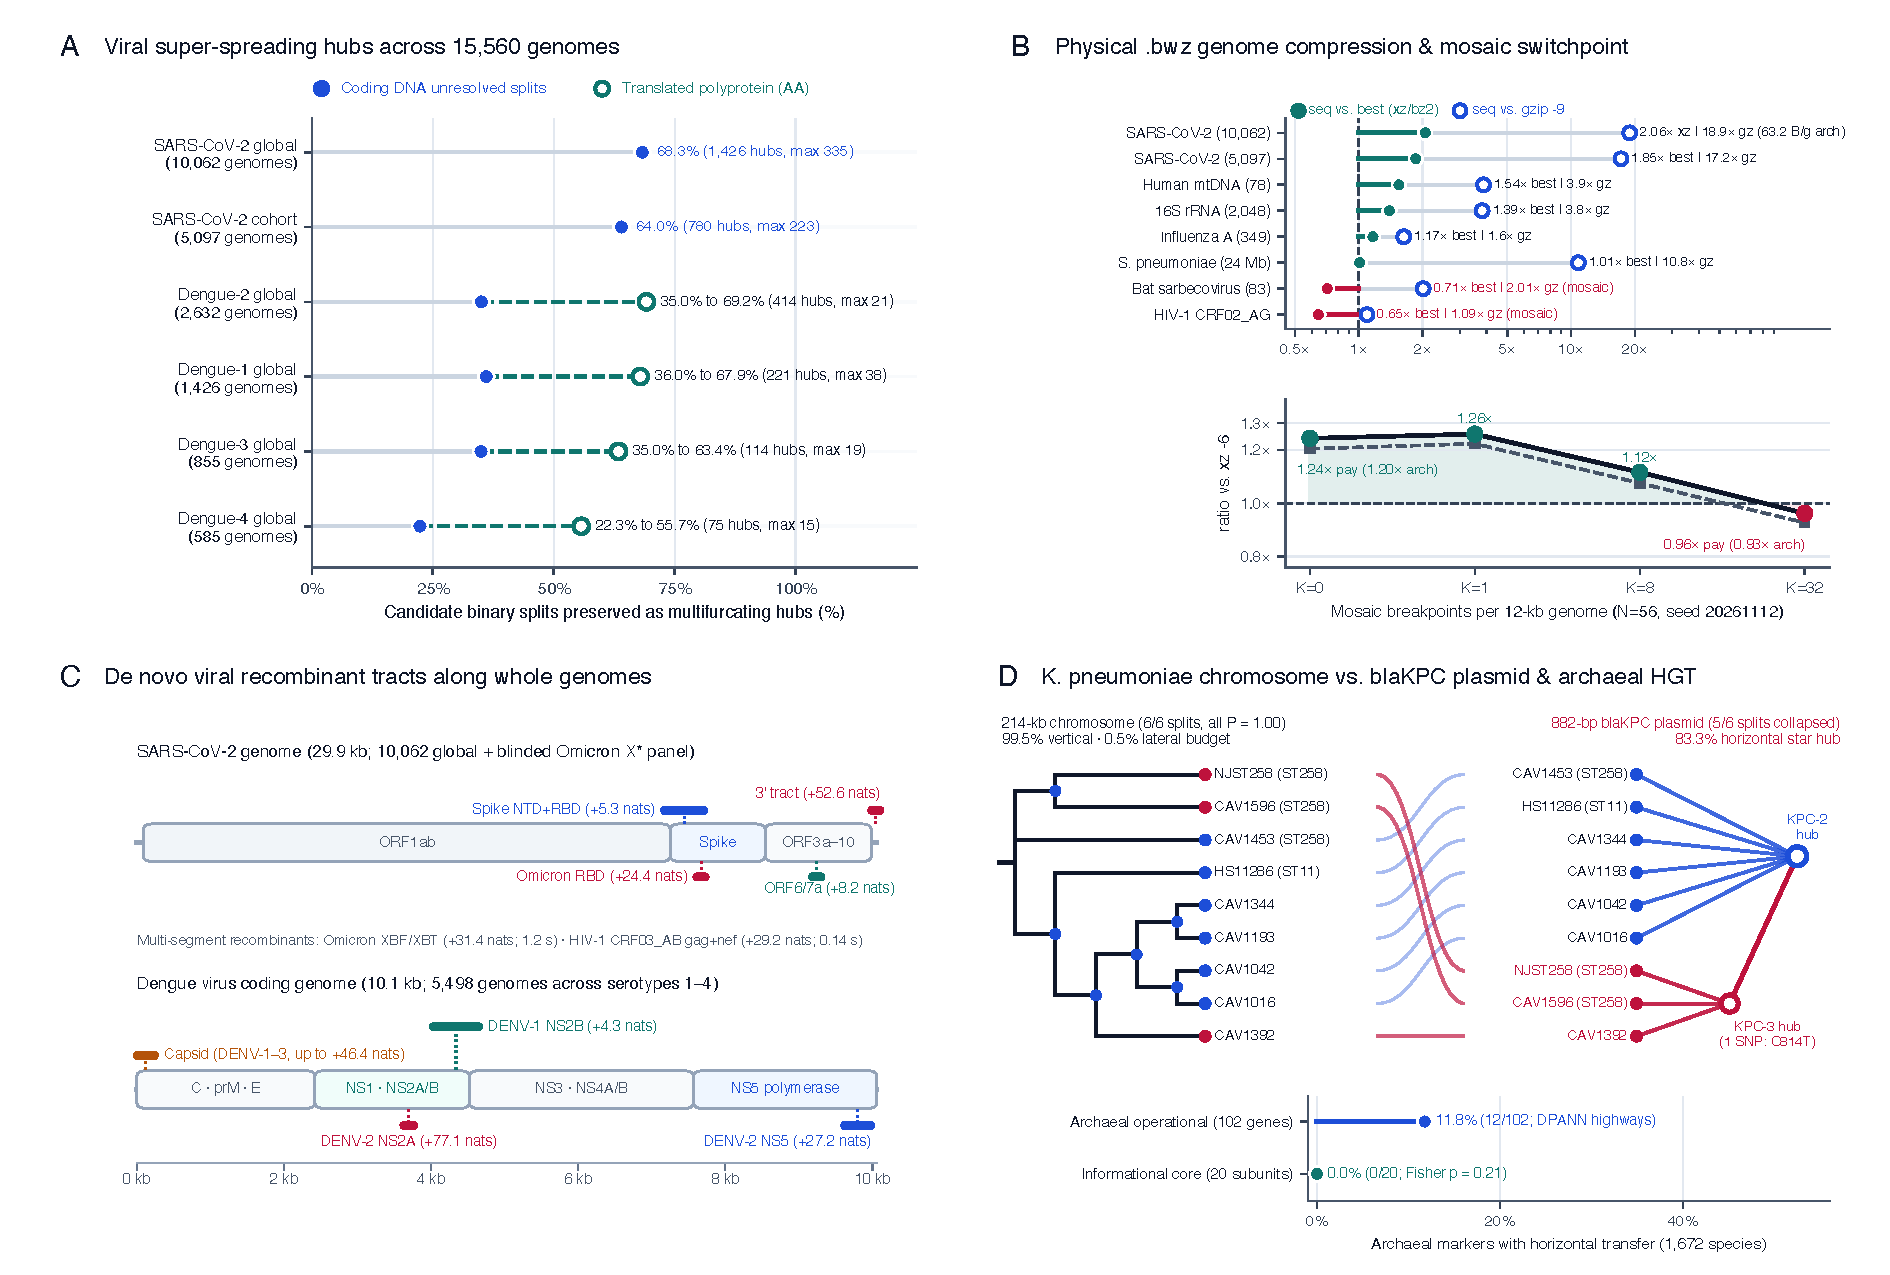
\includegraphics[width=\textwidth]{fig_science_microbial_viral.pdf}
\caption{\textbf{Viral superspreading hubs, physical genome compression, whole-genome recombinant mapping, and microbial gene-transfer budgets.} (\textbf{A}) Candidate binary splits preserved as multifurcating outbreak hubs and largest hub sizes across 10,062 global SARS-CoV-2 genomes ($68.3\%$ unresolved; 1,426 hubs up to 335 descendants) and 5,498 global dengue genomes across serotypes 1--4 in coding DNA versus translated polyproteins. (\textbf{B}) Physical lossless \texttt{.bwz} sequence payload and full archive size reductions over \texttt{xz -6}/\texttt{bzip2 -9} (up to $2.06\times$ sequence payload) and \texttt{gzip -9} (up to $18.9\times$ sequence payload; $38.5\text{ B/genome}$ payload and $63.2\text{ B/genome}$ total archive on SARS-CoV-2; top), contrasted with the crossover below $1\times$ under whole-genome mosaicism across controlled breakpoint titrations ($K = 0 \to 32$, $1.24\times \to 0.96\times$ payload, $1.20\times \to 0.93\times$ archive; bottom), bat sarbecoviruses ($0.71\times$), and recombinant HIV-1 ($0.65\times$). (\textbf{C}) Certified mosaic recombinant tracts mapped along the $29.9\text{-kb}$ SARS-CoV-2 and $10.1\text{-kb}$ dengue genomes in a single run. (\textbf{D}) Side-by-side tanglegram of nine carbapenem-resistant clinical \textit{Klebsiella pneumoniae} isolates on the $214\text{-kb}$ core chromosome ($6/6$ splits resolved at $P_{\text{local}} = 1.00$; $99.5\%$ vertical budget) versus their $882\text{-bp}$ \textit{blaKPC} carbapenemase plasmid ($5/6$ splits collapsed into horizontal \textit{blaKPC-2} and \textit{blaKPC-3} [\texttt{C814T}] star hubs; top), above horizontal transfer rates across 122 archaeal marker proteins in 1,672 species ($20.6\%$ operational versus $0.0\%$ informational core subunits, nominal two-sided Fisher $p = 0.0235$; bottom).}
\label{fig:microbial_viral}
\end{figure}

Encoding genome cohorts into lossless \texttt{.bwz} archives via arithmetic coding \citep{witten1987arithmetic} also tests directly whether shared descent is the main physical regularity of biological sequences (Fig.~\ref{fig:microbial_viral}B and Table~S9). Storing all $10,062$ SARS-CoV-2 genomes ($300.9\text{ MB}$ raw sequence) requires $636\text{ KB}$ for the complete archive ($63.2\text{ bytes}$ per viral genome; $1.25\times$ smaller than \texttt{xz -6} and $11.5\times$ smaller than \texttt{gzip -9}) and just $388\text{ KB}$ for the compressed sequence payload ($38.5\text{ bytes/genome}$; $2.06\times$ smaller than \texttt{xz -6} and $18.9\times$ smaller than \texttt{gzip -9}), with consistent gains across influenza, dengue, mitochondrial, plastid, and whole bacterial chromosomes. Equally telling is when that advantage reverses: across controlled recombination titrations ($K = 0 \to 32$, crossing from $1.24\times$ to $0.96\times$ payload relative to \texttt{xz -6}), mosaic bat sarbecoviruses ($0.71\times$) \citep{boni2020evolutionary,lytras2022exploring}, and recombinant HIV-1 ($0.65\times$), pervasive whole-genome mosaicism erases any single tree and lets multi-donor string dictionaries overtake single-tree coding, making archive size a direct gauge of tree-like versus mosaic evolution.

In prokaryotes, pricing vertical splits and horizontal transfers in the same unit turns qualitative debates over a microbial ``Tree versus Web of Life'' \citep{doolittle1999phylogenetic,parks2018gtdb} and the Complexity Hypothesis \citep{jain1999horizontal,woese2000aminoacyl} into a quantitative budget (Fig.~\ref{fig:microbial_viral}D and Table~S8). In hospital outbreaks of carbapenem-resistant \textit{Klebsiella pneumoniae} \citep{wyres2020population}, the $214\text{-kb}$ core chromosome resolves every branch across nine clinical isolates ($6/6$ splits at $P_{\text{local}} = 1.00$, with lateral transfer contributing just $0.5\%$ of the chromosomal budget), whereas the $882\text{-bp}$ \textit{blaKPC} plasmid carried by those exact same strains collapses $5$ of $6$ splits into multifurcating \textit{blaKPC-2} and \textit{blaKPC-3} star hubs separated by a single nucleotide (\texttt{C814T}) as horizontal plasmid spread outpaces mutation. Across 122 marker proteins in $1,672$ archaeal species \citep{parks2020gtdb}, horizontal transfers likewise appear in $20.6\%$ ($21/102$) of operational metabolic and regulatory genes---including cross-phylum highways between symbiotic DPANN archaea and their hosts \citep{castelle2018major}---versus $0\%$ ($0/20$, nominal two-sided Fisher $p = 0.0235$, $q = 0.027$) of core ribosomal and RNA polymerase subunits; and as single-gene microbiome 16S rRNA trees scale from $256$ to $32,768$ taxa \citep{mcdonald2012greengenes}, supported splits rise to $91.4\%$ ($N=1,024$) and saturate smoothly to $76.0\%$ ($N=32,768$), cutting mean taxonomy-contradicting splits per group by $19\%$ to $24\%$ relative to forced-binary resolution while running $4.5\times$ faster than \texttt{FastTreeMP} ($252\text{ s}$ versus $1,133\text{ s}$; Table~S1).

\subsection*{Somatic selection and clonal evolution in single cells}

Inside germinal centers and tumors, positively selected cells divide so rapidly that a single founder spawns a star-like burst of daughter lineages before new somatic mutations arise \citep{tas2016visualizing}. Whereas specialized lineage tools recover these bursts only when given cell-abundance counts or hypermutation models \citep{dewitt2018gctree}, reconstructing 147 mouse germinal centers ($10,429$ B cells across $29$ mice, $9,352$ unique genotypes \citep{dewitt2026gcreplay}) from deduplicated sequences alone shows that compression geometry reads out Darwinian selection directly (Fig.~\ref{fig:tree_scales}A,B and Table~S1).

\begin{figure}[t!]
\centering
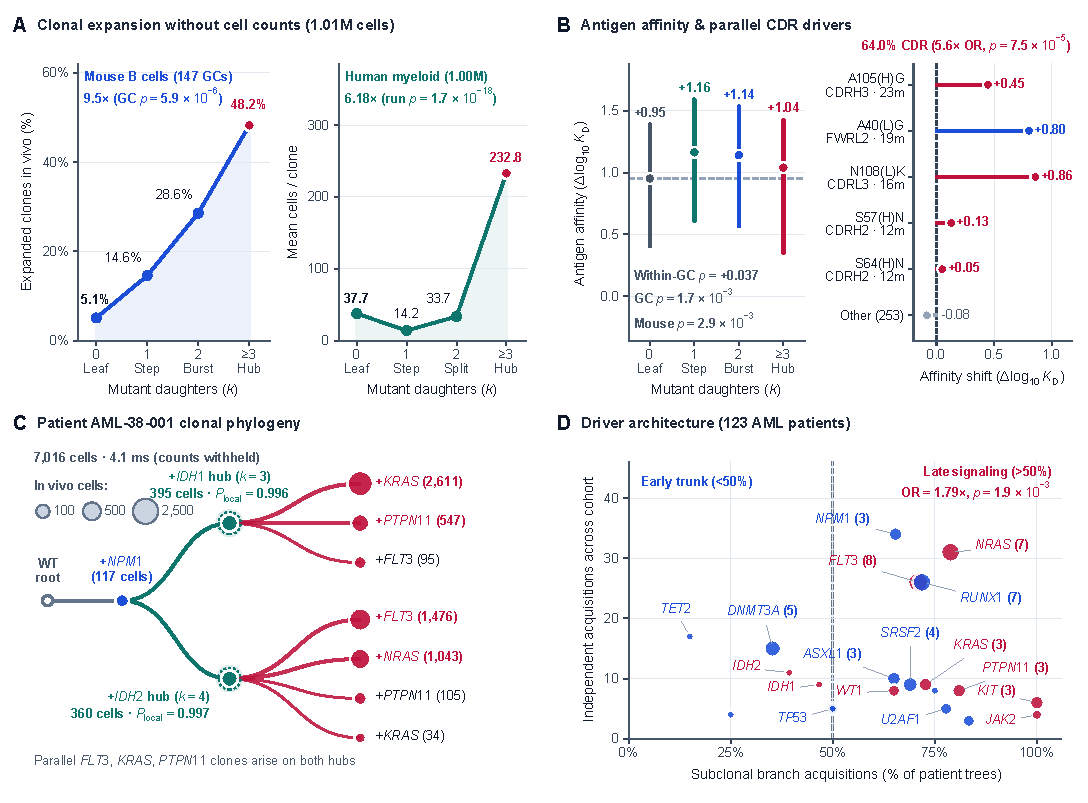
\includegraphics[width=\textwidth]{fig_science_tree_scales.pdf}
\caption{\textbf{Somatic compression hubs predict in vivo clonal selection and parallel resistance across single-cell immune repertoires and human leukemia.} (\textbf{A}) With all cell counts withheld during inference, inferred mutant daughter degree $k$ monotonically predicts in vivo clonal expansion across 147 mouse B-cell germinal centers ($10,429$ cells \citep{dewitt2026gcreplay}; $5.1\% \to 48.2\%$, $9.5\times$, hierarchical GC paired Wilcoxon $p = 5.9 \times 10^{-6}$; left) and 168 human myeloid single-cell DNA cohorts ($1,001,609$ cells; $37.7 \to 232.8$ mean cells per clone, $6.18\times$, per-run paired Wilcoxon $p = 1.7 \times 10^{-18}$; right). (\textbf{B}) Independent yeast-display antigen-binding affinity ($\Delta\log_{10} K_D$) across inferred B-cell node classes (hierarchical within-GC trend $p = 1.7 \times 10^{-3}$, within-mouse $p = 2.9 \times 10^{-3}$; left) and across parallel cross-mouse mutations ($64.0\%$ inside complementarity-determining regions versus $24.1\%$ background, $5.6\times$ odds ratio, $p = 7.5 \times 10^{-5}$; right). (\textbf{C}) Empirical single-cell leukemic clonal phylogeny of human patient \texttt{AML-38-001} ($7,016$ sequenced cells), reconstructed in $3.0\text{ ms}$ with cell counts withheld (circle area proportional to held-out in vivo cell count): an early \textit{NPM1} founder splits into parallel \textit{IDH1} ($P_{\text{local}} = 0.996$, $k = 3$) and \textit{IDH2} ($P_{\text{local}} = 0.997$, $k = 4$) burst hubs, each independently radiating subclonal \textit{FLT3}, \textit{KRAS}, \textit{NRAS}, and \textit{PTPN11} signaling resistance branches. (\textbf{D}) Clonal trunk-to-subclone driver architecture across all 123 acute myeloid leukemia patients, separating early epigenetic/chromatin founders from late subclonal signaling resistance drivers ($\text{OR} = 1.79\times$, two-sided Fisher $p = 1.9 \times 10^{-3}$; bubble size and numbers denote parallel within-patient acquisitions).}
\label{fig:tree_scales}
\end{figure}

Grouping B-cell genotypes solely by how many mutant daughter lineages ($k$) radiate from each node predicts a $9.5$-fold rise in in vivo clonal expansion from $k=0$ terminal leaves ($5.1\%$) to $k \ge 3$ burst hubs ($48.2\%$; hierarchical per-GC two-sided Wilcoxon $p = 5.9 \times 10^{-6}$, $q = 1.4 \times 10^{-5}$; per-mouse $p = 2.0 \times 10^{-6}$) and correlates significantly with tighter yeast-display antigen binding within germinal centers ($p = 1.7 \times 10^{-3}$, $q = 2.6 \times 10^{-3}$) and mice ($p = 2.9 \times 10^{-3}$, $q = 3.9 \times 10^{-3}$), while parallel cross-mouse mutations ($\ge 5$ mice) enrich $5.6$-fold inside antigen-contacting complementarity-determining regions ($64.0\%$ versus $24.1\%$, $p = 7.5 \times 10^{-5}$, $q = 1.6 \times 10^{-4}$; $+0.31$ versus $-0.08\;\Delta\log_{10} K_D$, $p = 8.1 \times 10^{-5}$; Fig.~\ref{fig:tree_scales}A,B).

Extending the same framework beyond DNA sequences to somatic mutation and copy-number profiles in human cancer---with all cell counts and clinical labels withheld---reveals the same selective signature in patient tumors (Fig.~\ref{fig:tree_scales}A,C,D, Fig.~S6, and Table~S10). In a single leukemia patient (\texttt{AML-38-001}, $7,016$ sequenced cells; Fig.~\ref{fig:tree_scales}C), reconstructing clonal history in $3.0\text{ ms}$ recovers an early \textit{NPM1} founder that splits into parallel \textit{IDH1} ($P_{\text{local}} = 0.996$, $k=3$) and \textit{IDH2} ($P_{\text{local}} = 0.997$, $k=4$) burst hubs, each independently radiating three to four subclonal \textit{FLT3}, \textit{KRAS}, \textit{NRAS}, and \textit{PTPN11} resistance branches. Across all $168$ COMPASS myeloid single-cell cohorts ($129$ patients, $1.00\text{ million}$ cells \citep{sollier2023compass}), inferred burst hubs ($k \ge 3$) carry $6.18$-fold more leukemic cells in vivo than terminal leaves ($232.8$ versus $37.7$ cells; per-run paired Wilcoxon $p = 1.7 \times 10^{-18}$, $q = 1.9 \times 10^{-17}$; per-patient $p = 3.5 \times 10^{-14}$) and resolve $90.3\%$ ($2,858/3,164$) stepwise CN-LOH transitions; across the separate $123$-patient Morita AML cohort \citep{morita2020clonal}, branching hubs spawn significantly larger descendant lineages ($n=97$, paired Wilcoxon $p = 3.0 \times 10^{-15}$, whereas direct hub cell multiplicity is null at $p = 0.20$) while late subclonal signaling resistance drivers enrich relative to early epigenetic founders ($\text{OR} = 1.79$, two-sided Fisher $p = 1.9 \times 10^{-3}$, $q = 2.7 \times 10^{-3}$) and recur in parallel within $44$ patients (Fig.~\ref{fig:tree_scales}A,D). On $4,950$ single-cell whole-genome copy-number profiles across ovarian and breast tumors \citep{salehi2023sitka}, ordered step coding compresses raw $500\text{-kb}$ genomes $21.9$- to $33.5$-fold ($21.9\text{ s}$ on colinear segments; $113.6\text{ s}$ on raw bins), contracting $39\text{--}53\%$ of noisy splits while preserving cohort clade purity ($57.9\%\text{--}95.7\%$ versus $20.8\%\text{--}59.9\%$ random null and $60.1\%\text{--}96.7\%$ forced-binary; \texttt{OV2295} ovarian tumor versus ascites $95.7\%$ purity, $F_1 = 0.997$ segment / $0.995$ bin).

\subsection*{Outlook}

Viewing evolutionary inference as lossless compression shows that tree topology, branch support, evolutionary rates, gene transfer, and adaptive convergence follow from a single principle: shared descent shortens the description of biological variation. Because every branch or lateral link must pay its own cost in information, unresolved hubs become a quantitative biological signal rather than a statistical failure---marking rapid species radiations, epidemic superspreading, and Darwinian clonal bursts in immunity and cancer without arbitrary cutoffs. Pricing lateral links in the same currency separates local gene conversion from cross-order convergence and turns debates over microbial gene transfer into genome-wide budgets, while scaling Tree-of-Life phylogenies to standard laptops and web browsers. Because this principle requires only heritable states copied with sparse changes, it extends naturally beyond sequences and somatic profiles to epigenetic marks, CRISPR lineage barcodes, and morphological or linguistic characters wherever history leaves a compressible trace.

% ============================================================================
% References and Notes + Science Back-Matter
% ============================================================================

\bibliographystyle{unsrtnat}
\bibliography{references}

\section*{Acknowledgments}
\noindent\textbf{Funding:} Supported by grants from the National Institutes of Health and the National Science Foundation (S.L.K.P. and A.N.).\\
\textbf{Author contributions:} Conceptualization: S.L.K.P., D.P.M., A.N. Methodology and software: S.L.K.P., D.P.M., S.J.K.P. Investigation, validation, and visualization: S.L.K.P., D.P.M., S.J.K.P., A.N. Writing---original draft and review \& editing: S.L.K.P., D.P.M., S.J.K.P., A.N.\\
\textbf{Competing interests:} The authors declare that they have no competing interests.\\
\textbf{Data and materials availability:} The open-source Rust and WebAssembly implementation of Bushwhacker (supporting nucleotide, amino-acid, binary, and discrete/ordered character matrices), the \texttt{.bwz} lossless archival codec, interactive browser application (\url{https://veg.github.io/bushwacker/}), reproducibility scripts, and empirical and ground-truth validation ledgers spanning more than $81{,}000$ empirical alignments, $1.01$ million single cells, and $36{,}920$ simulated evolutionary histories are available at \url{https://github.com/veg/bushwacker} and bundled in the Zenodo v1.0 replication archive (\texttt{bushwhacker\_science\_zenodo\_v1.0}, containing source code, specimens, assembled alignments, all JSON/CSV benchmark ledgers, figure scripts, and automated downloaders for external public archives; see Materials and Methods for complete accessions and DOIs).

\section*{Supplementary Materials}
\noindent Materials and Methods\\
Supplementary Text\\
Figs.~S1 to S6\\
Tables~S1 to S11\\
References (\textit{63}--\textit{88})

\end{document}
